
\section{Shallow Ice Test Cases}

These tests are primarily useful for testing the shallow ice approximation (SIA) dycore, Glide.


% =====================================
\subsection{Halfar dome}
% =====================================

\label{sec:halfar_description}
This test case describes the time evolution of a dome of ice as described by \citet{Halfar1983}.
This test provide an analytic solution for a flat-bedded SIA problem.

\begin{equation}
    \label{halfar}
    \frac{\partial H}{\partial t} = \nabla \cdot (\Gamma H^{n+2} |\nabla H|^{n-1} \nabla H)
\end{equation}
where $n$ is the exponent in the Glen flow law, commonly taken as 3, and $\Gamma$ is a positive constant:
\begin{equation}
    \Gamma = \frac{2}{n+2} A (\rho g)^n
\end{equation}

For $n=3$, this reduces to:
\begin{equation}
    H(t,r) = H_0 \left(\frac{t_0}{t}\right)^\frac{1}{9}  \left[ 1 - \left(  \left( \frac{t_0}{t} \right) ^ \frac{1}{18} \frac{r}{R_0} \right)^\frac{4}{3} \right] ^ \frac{3}{7}
\end{equation}
where
\begin{equation}
    t_0 = \frac{1}{18\Gamma} \left( \frac{7}{4} \right)^3 \frac{R_0^4}{H_0^7}
\end{equation}
and $H_0, R_0$ are the central height of the dome and its radius at time $t=t_0$.

For more details see \url{http://www.projects.science.uu.nl/iceclimate/karthaus/2009/more/lecturenotes/EdBueler.pdf},  \citet{Bueler2005}, \citet{Halfar1983}.



\subsubsection{Provided Files}
\label{subsec:halfar_files}

Our implementation of the Halfar dome has an initial radius of $R_0=21.2$ km and an initial thickness of $H=707.1$ m.
These values can be changed by editing \texttt{halfarDome.py}.

\begin{itemize}
	\item README \\
		Information about the test case.
	\item halfar.config \\
		This is the config file defining CISM options. \\
    There is also a version named \texttt{halfarHO.config} that is setup to run the Glissade dycore.
	\item halfar.py \\
		This python script generates the dome initial condition and \\
		runs CISM.
	\item halfar\_results.py \\
		This is script compares model results to the analytic solution.
	\item halfarDome.py \\
		This is a python module that defines the analytic solution. \\
    It is not meant to be run manually, but it is imported by the other scripts.
\end{itemize}

\subsubsection{Results}
\label{subsecc:halfar_results}
With the default .config settings, this simulation should only take a few seconds and is a good first test for a working Glide dycore.
As the dome of ice evolves, its margin advances and its thickness decreases (there is no surface mass balance to add new mass).  The script \texttt{halfar\_results.py} will plot the modeled and analytic thickness at a specified time (Figure \ref{fig:halfarresults}), as well as report model error statistics.  Invoke \texttt{halfar\_results.py --help} for details of its usage.


\begin{figure}[H!]
	\centering
	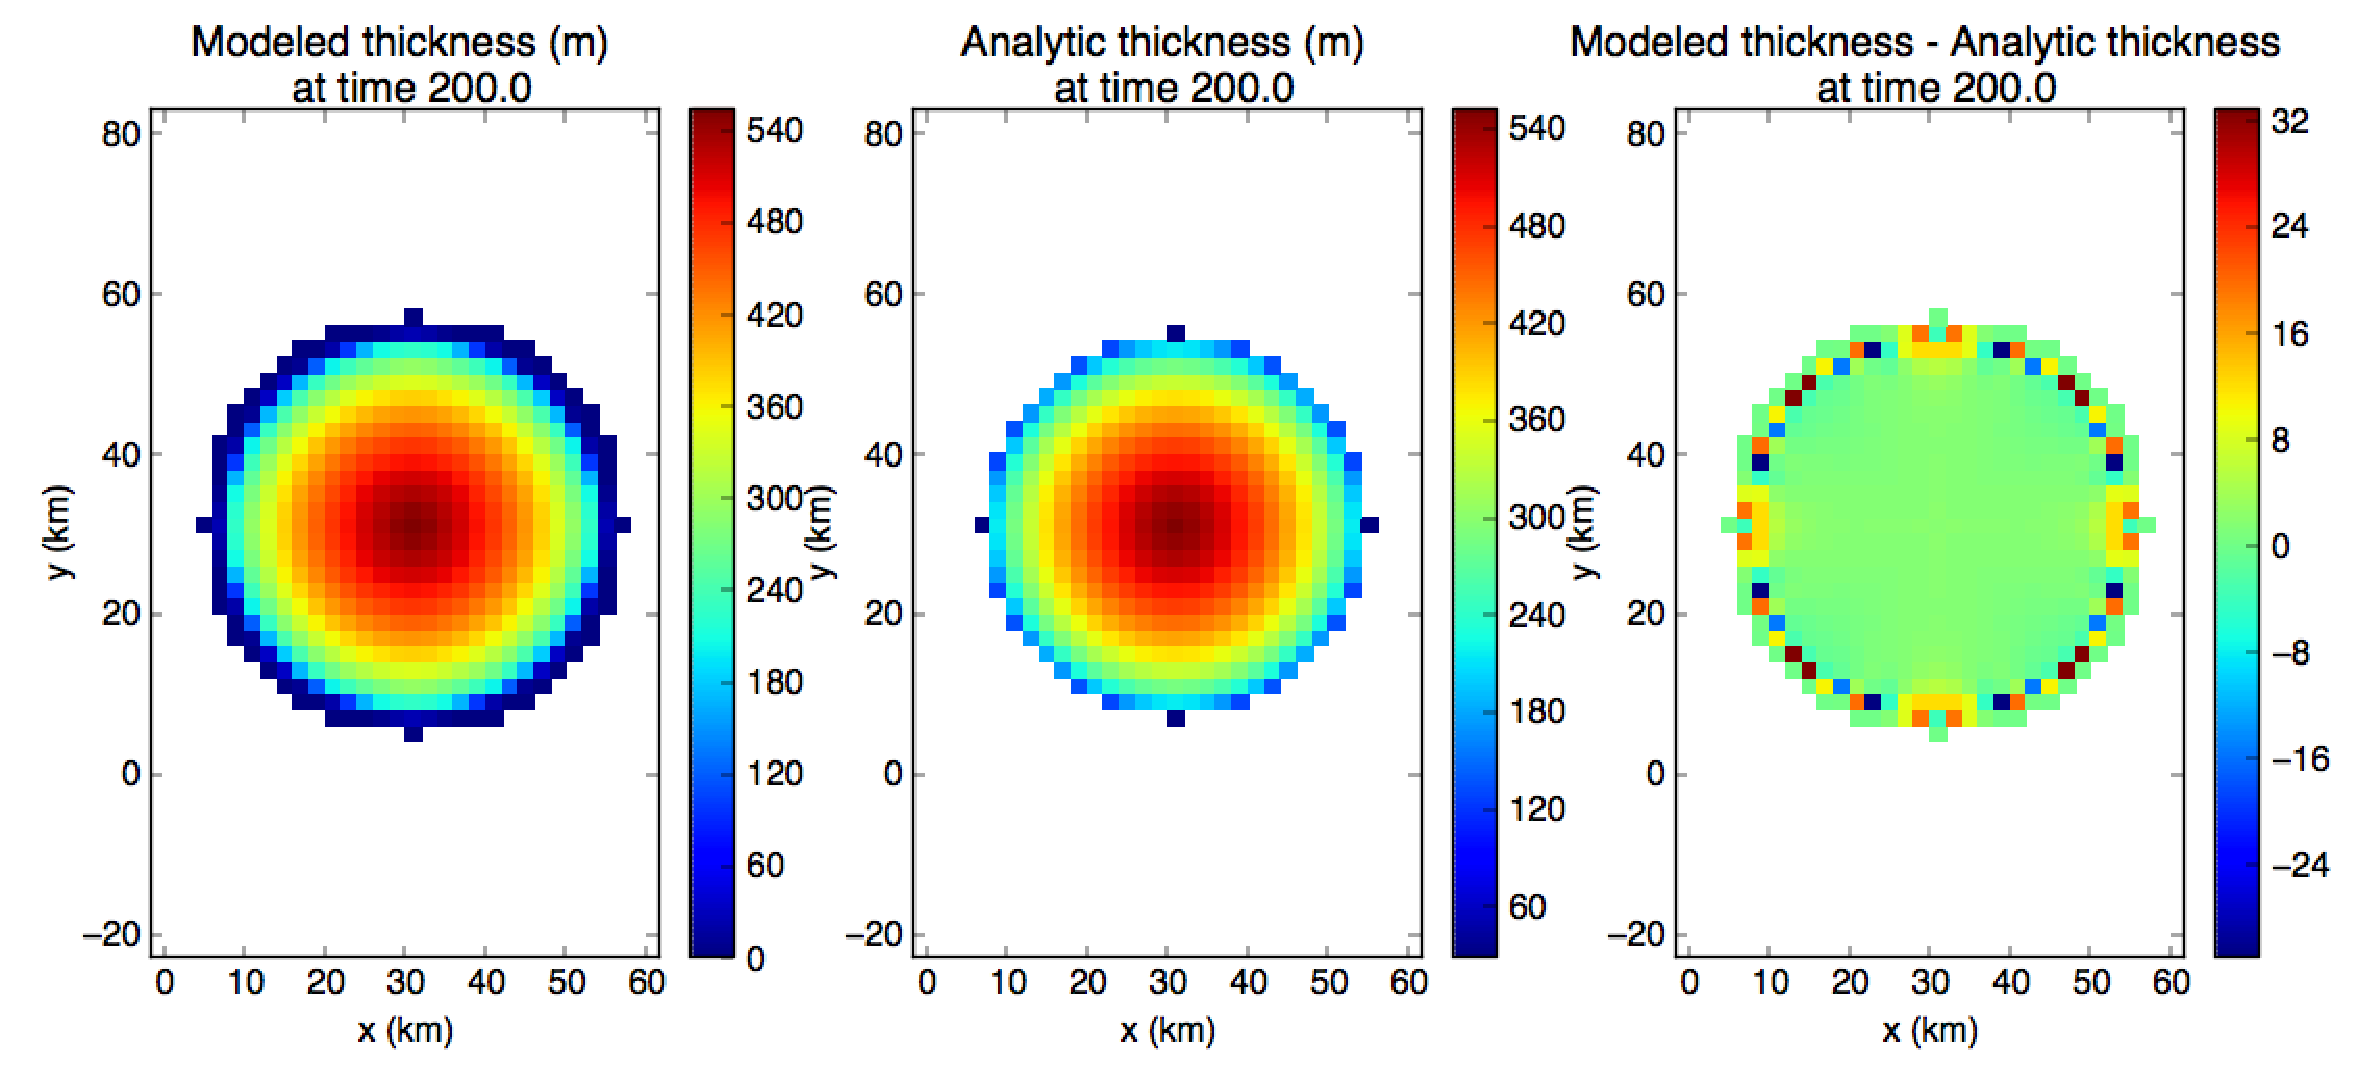
\includegraphics[width=16.4cm]{\dir/halfar_results.eps}
	\caption{Halfar test case results after 200 years of dome evolution. This figure is generated by \texttt{halfar\_results.py}.}
	\label{fig:halfarresults}
\end{figure}


\FloatBarrier


% =====================================
\subsection{EISMINT-1}
% =====================================
\label{sec:eismint_description}
This test case is from phase 1 of the European Ice Sheet Modelling INiTiative intercomparison experiments.  These experiments are described at \url{http://homepages.vub.ac.be/~phuybrec/eismint.html} and in \citet{Huybrechts1996}.

\subsubsection{Provided Files}
\label{subsec:eismint_files}

\begin{itemize}
	\item README \\
		Information about the test case.
\item *.config \\
  There are six .config files for each of the six experiments in EISMINT 1.  There are three fixed margin experiments (fm) and three moving margin experiments (mm).
\end{itemize}


\subsubsection{Results}
\label{subsecc:eismint_results}
There is not a script for running these experiments.  They must be run manually, e.g.: 

\texttt{./cism\_driver e1-fm.1.config}

These experiments are meant to be run to steady-state, and the supplied .config files are setup to run for long enough for it to be reached.
These simulations take more than a few minutes to complete.
As the initial ice sheet evolves, its shape eventually reaches a steady-state with the imposed surface mass balance.  Currently there is not a script for analyzing the CISM results.  Users can manually compare their results to those in the \citet{Huybrechts1996} paper.


% =====================================
\subsection{EISMINT-2}
% =====================================
\label{sec:eismint2_description}
This test case is from phase 2 of the European Ice Sheet Modelling INiTiative intercomparison experiments.  These experiments are described at \url{http://homepages.vub.ac.be/~phuybrec/eismint.html} and in \citet{Payne2000}.

\subsubsection{Provided Files}
\label{subsec:eismint2_files}

\begin{itemize}
	\item README \\
		Information about the test case.
  \item *.config \\
  There are 11 .config files for each of the a-f experiments in EISMINT-2.
  \item mound.nc, trough.nc \\
    These are input netCDF files used by the EISMINT-2 experiments.
\end{itemize}


\subsubsection{Results}
\label{subsecc:eismint2_results}
There is not a script for running these experiments.  They must be run manually, e.g.: 

\texttt{./cism\_driver e2.a.config}

These experiments are meant to be run to steady-state, and the supplied .config files are setup to run for long enough for it to be reached.  
Note that some of the experiments use the final state of a previous experiment 
as the initial condition.  See experiment descriptions in \citet{Payne2000} for details.
These simulations take more than a few minutes to complete.
As the initial ice sheet evolves, its shape eventually reaches a steady-state with the imposed surface mass balance.  Currently there is not a script for analyzing the CISM results.  Users can manually compare their results to those in the \citet{Payne2000} paper.


% =====================================
\subsection{GLINT example}
% =====================================



